\chapter{Background} \label{sec:methods}
\section{Skinned Multi-Person Linear Model (SMPL)}
\begin{figure}[h]
    \centering
    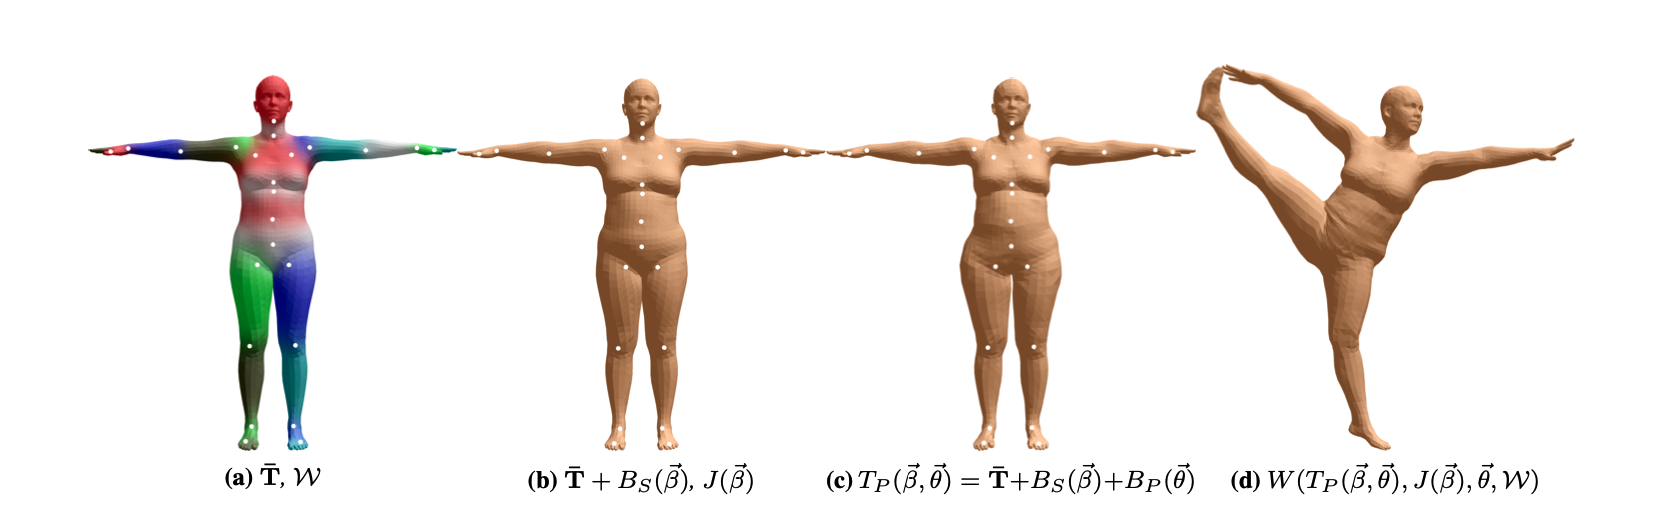
\includegraphics[width=\linewidth]{figures/smpl.png}
    \caption{SMPL model}
\end{figure}
The Skinned Multi-Person Linear (SMPL) model is a parametric body shape model that accurately represents a wide range of human bodies and poses. It is built upon a foundation of linear blend skinning enhanced with corrective blend shapes, which are derived from a large dataset of body scans. The model captures the subtle deformations that occur with different body shapes and poses and can easily be rendered due to its compatibility with existing graphics pipelines. Since its publication, several extensions such as DMPL, incorporating dynamic soft-tissue deformation and SMPL-X, also modelling hands and facial expressions have been introduced. The model is parameterized by $\vec{\beta}$, capturing the variations from a mean body shape and $\vec{\theta}$, specifying the axis-angle rotation of 23 of the template skeleton joints. Mathematically, the model can be expressed as:
\begin{equation}
    M(\vec{\beta}, \vec{\theta}) = W(T_P(\vec{\beta}, \vec{\theta}), J(\vec{\beta}), \vec{\theta}, \mathcal{W})
\end{equation}
where $T_P(\vec{\beta}, \vec{\theta})$ returns the vertices of the rest pose, incorporating the deformations from the body shape and pose and is given by:
\begin{equation}
    T_P(\vec{\beta}, \vec{\theta}) = \vect{\bar{T}} + B_S(\vec{\beta}) + B_P(\vec{\theta})
\end{equation}
$J(\vec{\beta})$ returns the 3D joint locations from the shaped template vertices using a learned regression matrix $\mathcal{J}$ and is given by:
\begin{equation}
    J(\vec{\beta}) = \mathcal{J}(\vect{\bar{T}} + B_S(\vec{\beta}))
\end{equation}
$W$ is the skinning function (e.g. Linear Blend Skinning (LBS) or Dual-Quaternion Blend Skinning (DQBS)) and $\mathcal{W}$ is the blend weights. 

\section{Human Mesh Reconstruction (HMR)}
Recovering the mesh of humans have several applications\dots

\section{Denoising Diffusion Probabilistic Models (DDPM)}

In recent years, several types of generative models such as Variational Autoencoders (VAEs), Generative Adverserial Networks (GANs), autoregressive models and flow-based models have shown remarkable results in data generation of varying data modalities, such as images, audio, videos and text. Most recently, Denoising Diffusion Probabilistic Models (DDPMs) have gained large popularity especially within the field of image generation due to several reasons such as high-quality data generation, versitility in several data domains as well as controllability, allowing one to steer the generation towards desired outputs.
A DDPM is a parametarized ($\theta$) Markov chain trained using variational inference to reverse a (forward) diffusion process, $q(\vect{x}_{1:T} \mid \vect{x}_0)$ wherein the signal of the data, $\vect{x}_0$, is gradually destroyed by adding gaussian noise according to predefined noise schedule $\{\beta_t  \in (0,1) \}_{t=1}^T$ giving rise to increasingly noisy samples, $\vect{x}_1 \ldots \vect{x}_T$. The forward process is defined as follows:
\begin{equation}    
    q(\vect{x}_{1:T} \mid \vect{x}_{0}) = \prod_{t=1}^T q(\vect{x}_{t} \mid \vect{x}_{t-1}), \quad q(\vect{x}_{t} \mid \vect{x}_{t-1}) = \mathcal{N}(x_{t}; \sqrt{1 - \beta_t}\vect{x}_t,\beta_t \vect{I} )
\end{equation}
with $T$ being the discritized number of diffusion steps before all original information is completely discarded. The goal of the inverse or backwards process then becomes to iteratively remove the noise, in order to arrivate at the original data. More formally, the process is defined as:
\begin{equation}
    p_\theta(\vect{x}_{0:T}) = p(\vect{x}_T) \prod_{t=1}^T p_\theta(\vect{x}_{t-1} \mid x_{t}), \quad p_\theta(\vect{x}_{t-1} \mid \vect{x}_{t}) = \mathcal{N}\left(\vect{x}_{t-1}; \vect{\mu}_\theta(\vect{x}_t, t), \vect{\Sigma}_\theta(\vect{x}_t, t) \right)
\end{equation}
taking starting point in pure noise $p(\vect{x}_T) = \mathcal{N}(\vect{x}_T; \vect{0}, \vect{I})$, incrementally removing the noise through the learned functions, $\vect{\mu}_\theta(\vect{x}_t, t)$ and $\vect{\Sigma}_\theta(\vect{x}_t, t)$ commonly parameterized by a deep neural network.
Using the reparameterization trick, we are able to sample any noisy version of our data, $\vect{x}_t$, at time step $t$ given our original data $\vect{x}_0$. Recall our forward transition probability function, $q(\vect{x}_t \mid \vect{x}_{t-1})$. Letting $\alpha_t = 1 - \beta_t$, $\bar{\alpha}_t = \prod_{i=1}^t \alpha_i$ and using the reparameterization trick the expression can be rewritten as:
\begin{equation}
    \vect{x}_t = \sqrt{\alpha_t} \vect{x}_{t-1} + \sqrt{1 - \alpha_t} \epsilon_{t-1}
\end{equation}
where $\epsilon_{t-1} \sim \mathcal{N}(0,1)$. Expanding the recursive definition then gives:
\begin{align*}
    \vect{x}_t    & = \sqrt{\alpha_t} \vect{x}_{t-1} + \sqrt{1 - \alpha_t} \vect{\epsilon_{t-1}} \\
                    & = \sqrt{\alpha_t} \left(
    \sqrt{\alpha_{t-1}} \vect{x}_{t-2} + \sqrt{1 - \alpha_{t-1}} \vect{\epsilon}_{t-2}
    \right) + \sqrt{1 - \alpha_t} \vect{\epsilon_{t-1}} \\
                    & = \sqrt{\alpha_t \alpha_{t-1}} \vect{x}_{t-2} + \sqrt{\alpha_t(1 - \alpha_{t-1})} \vect{\epsilon_{t-2}} + \sqrt{1 - \alpha_{t}} \vect{\epsilon_{t-1}} \\
                    & = \sqrt{\alpha_t \alpha_{t-1}} \vect{x}_{t-2} + \sqrt{1 - \alpha_{t}\alpha_{t-1}} \vect{\bar{\epsilon}}_{t-2}
\end{align*}
where $\vect{\bar{\epsilon}}_{t-2}$ merges the two independent Gaussians $\vect{\epsilon}_{t-1}$ and $\vect{\epsilon}_{t-2}$ into a single Gaussian with new variance as the sum of variances $\alpha_t (1 - \alpha_{t-1}) + (1 - \alpha_{t}) = 1 - \alpha_t \alpha_{t-1}$. Recursively applying the definition of $\vect{x}_t$ and merging the gaussian noise terms results in the simplified expression:
\begin{equation} \label{eq:nice}
    \vect{x}_t = \sqrt{\bar{\alpha}_t}\vect{x}_0 + \sqrt{1 - \bar{\alpha}_t} \vect{\epsilon}, \quad \vect{\epsilon} \sim \mathcal{N}(\vect{0}, \vect{I})
\end{equation}
% or by undoing the reparameterization:
% \begin{equation}
%     q(\vect{x}_t \vert \vect{x}_0) = \mathcal{N}(\vect{x}_t; \sqrt{\bar{\alpha}_t} \vect{x}_0, (1 - \bar{\alpha}_t)\vect{I})
% \end{equation}
%This result enables sampling of any noisy version of $\vect{x}_t$ at time $t$ given "clean" data $\vect{x}_0$. 
Conversely, given $\vect{x}_0$ the reverse conditional probability:
\begin{equation*}
    q(\vect{x}_{t-1} \vert \vect{x}_t, \vect{x}_0) = \mathcal{N}\left( \vect{x}_{t-1}; \vect{\tilde{\mu}}_t(\vect{x}_t, \vect{x}_0), \tilde{\beta}_t \vect{I} \right)
\end{equation*}
becomes tractable to compute using Bayes rule (derivation in \cref{appendix:q-posterior-derivation}) with mean and variance given by:
\begin{align} \label{eq:x-t-min-1-from-x-t}
    \vect{\tilde{\mu}}_t(\vect{x}_t, \vect{x}_0) &= \frac{\sqrt{\bar{\alpha}_{t-1}} \beta_t}{1-\bar{\alpha}_t} \vect{x}_0+\frac{\sqrt{\alpha_t}\left(1-\bar{\alpha}_{t-1}\right)}{1-\bar{\alpha}_t} \vect{x}_t \overset{\text{Using \ref{eq:nice}}}{=} \frac{1}{\sqrt{\alpha_t}}\left(\vect{x}_t-\frac{1-\alpha_t}{\sqrt{1-\bar{\alpha}_t}} \vect{\epsilon}_t\right) \\
    \tilde{\beta}_t &= \frac{1-\bar{\alpha}_{t-1}}{1-\bar{\alpha}_t} \beta_t
\end{align}
The model is trained by optimizing the variational lower bound on the log likelihood:
\begin{equation}
    L_{VLB}
        = \mathbb{E}_q\left[ \log \frac{p_\theta(\vect{x}_{0:T})}{q(\vect{x}_{1:T} \vert \vect{x}_0)}\right]
        = \mathbb{E}_q\left[\log p(\vect{x_T}) + \sum_{t \geq 1} \log \frac{p_\theta(\vect{x}_{t-1} \vert \vect{x}_{t})}{q(\vect{x}_t \vert \vect{x}_{t-1})}
        \right]
        \leq \mathbb{E}\left[\log p_\theta(\vect{x}_0)\right]
\end{equation}
which in practice means minimizing the negative variational lower bound. 
\cite{ho2020denoising} rewrites this into a sum of KL-divergences:
\begin{equation}
    L_{VLB} = \mathbb{E}_q \left[ \underbrace{D_{\mathrm{KL}} \left(
            q\left(\vect{x}_T \mid \vect{x}_0\right) \| p_\theta\left(\vect{x}_T\right)
            \right)}_{L_T} + \sum_{t=2}^T \underbrace{D_{\mathrm{KL}}\left(q\left(\vect{x}_{t-1} \mid \vect{x}_t, \vect{x}_0\right) \| p_\theta\left(\vect{x}_{t-1} \mid \vect{x}_t\right)\right)}_{L_{t-1}} - \underbrace{\log p_\theta\left(\vect{x}_0 \mid \vect{x}_1\right)}_{L_0} \right]
\end{equation}
where $L_0$ is modelled from a seperate discrete decoder. The rest of the terms can be efficiently computed in the closed form, by fixing the variance $\vect{\Sigma}_\theta(\vect{x}_t, t) = \sigma_t^2 \vect{I}$ to only depend on the current timestep (authors propose $\sigma_t^2 = \beta_t$ or $\sigma_t^2 = \tilde{\beta}_t$). $L_{t-1}$ can then be written in closed form (derivation in \cref{appendix:L-closed-form}) as:
\begin{equation}
    L_{t-1} = \mathbb{E}_q \left[ \frac{1}{2\sigma_t^2} \| \vect{\tilde{\mu}}_t(\vect{x}_t, \vect{x}_0) - \vect{\mu}_\theta(\vect{x}_t, t) \|^2 \right] + C_t
\end{equation}
where $C_t$ is a constant depending on the choice of $\sigma_t^2$ and the noise schedule. Using \cref{eq:x-t-min-1-from-x-t} \cite{ho2020denoising} reparameterize the expression in terms of predicting the noise:
\begin{equation}
    L_{t-1} = \mathbb{E}_{\vect{x}_0, \vect{\epsilon}}\left[
        \frac{\beta_t^2}{2 \sigma_t^2 \alpha_t \left( 1 - \bar{\alpha}_t\right)} \left\| 
            \vect{\epsilon}-\vect{\epsilon}_\theta \left(\sqrt{\bar{\alpha}_t} \vect{x}_0+\sqrt{1-\bar{\alpha}_t} \vect{\epsilon}, t\right)
            \right\|^2
    \right]
\end{equation}
as they find it leads to better unconditional sample quality when training on the CIFAR10 dataset. Furthermore, they report the best sample quality when using the "simple" objective, ignoring the weighing:
\begin{equation} \label{eq:ddpm-simple-objective}
    L_\mathrm{simple} = \mathbb{E}_{t \sim \mathcal{U}(1, T),\ \vect{\epsilon}} \left[
        \vect{\epsilon} - \vect{\epsilon}_\theta( \sqrt{\bar{\alpha}} \vect{x}_0 + \sqrt{1 - \bar{\alpha}}\vect{\epsilon}, t)
    \right]
\end{equation}


\subsection{Cosine variance schedule}
As an alternative to the linear variance schedule introduced by \cite{ho2020denoising}... 

\subsection{Classifier-free Guidance (CFG)}


\section{Tranformer architecture}

\section{Human Motion Generation}
Generating realistic human motion has several applications 


- Human Motion Diffusion
- 


